\subsection*{Sequential characterization proposal}

\begin{figure}[H]
\centering

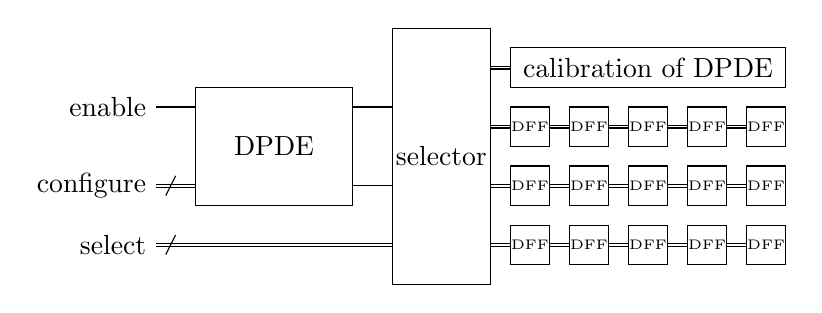
\begin{tikzpicture}

% DPDE and input
\draw  (-3,0.5) rectangle (-1,-1) node[pos=.5]{DPDE};
\draw [double] (-3.5,-0.75) -- (-3,-0.75);
\draw [] (-3,0.25) -- (-3.5,0.25);

\node [anchor=east] at (-3.5,0.25) {enable};
\node [anchor=east] at (-3.5,-0.75) {configure};
\draw (-3.375,-0.875) -- (-3.25,-0.625);

% select circuit
\draw  (-0.5,1.25) rectangle (0.75,-2) node[pos=.5]{selector};
\draw 
(-1,0.25) -- (-0.5,0.25)
(-1,-0.75) -- (-0.5,-0.75);
\draw [double] (-3.5,-1.5) -- (-0.5,-1.5);

\node [anchor=east] at (-3.5,-1.5) {select};
\draw (-3.375,-1.625) -- (-3.25,-1.375);

% calibration
\draw  (1,1) rectangle (4.5,0.5) node[pos=.5]{calibration of DPDE};
\draw [double](0.75,0.75) -- (1,0.75);

% FF chain
\draw  (1,0.25) rectangle (1.5,-0.25) node[pos=.5]{\tiny{DFF}};
\draw  (1.75,0.25) rectangle (2.25,-0.25) node[pos=.5]{\tiny{DFF}};
\draw  (2.5,0.25) rectangle (3,-0.25) node[pos=.5]{\tiny{DFF}};
\draw  (3.25,0.25) rectangle (3.75,-0.25) node[pos=.5]{\tiny{DFF}};
\draw  (4,0.25) rectangle (4.5,-0.25) node[pos=.5]{\tiny{DFF}};
\draw [double]
(0.75,0) -- (1,0)
(1.5,0) -- (1.75,0)
(2.25,0) -- (2.5,0)
(3,0) -- (3.25,0)
(3.75,0) -- (4,0);

% FF chain
\draw  (1,-0.5) rectangle (1.5,-1) node[pos=.5]{\tiny{DFF}};
\draw  (1.75,-0.5) rectangle (2.25,-1) node[pos=.5]{\tiny{DFF}};
\draw  (2.5,-0.5) rectangle (3,-1) node[pos=.5]{\tiny{DFF}};
\draw  (3.25,-0.5) rectangle (3.75,-1) node[pos=.5]{\tiny{DFF}};
\draw  (4,-0.5) rectangle (4.5,-1) node[pos=.5]{\tiny{DFF}};
\draw [double]
(0.75,-0.75) -- (1,-0.75)
(1.5,-0.75) -- (1.75,-0.75)
(2.25,-0.75) -- (2.5,-0.75)
(3,-0.75) -- (3.25,-0.75)
(3.75,-0.75) -- (4,-0.75);

% FF chain
\draw  (1,-1.25) rectangle (1.5,-1.75) node[pos=.5]{\tiny{DFF}};
\draw  (1.75,-1.25) rectangle (2.25,-1.75) node[pos=.5]{\tiny{DFF}};
\draw  (2.5,-1.25) rectangle (3,-1.75) node[pos=.5]{\tiny{DFF}};
\draw  (3.25,-1.25) rectangle (3.75,-1.75) node[pos=.5]{\tiny{DFF}};
\draw  (4,-1.25) rectangle (4.5,-1.75) node[pos=.5]{\tiny{DFF}};
\draw [double]
(0.75,-1.5) -- (1,-1.5)
(1.5,-1.5) -- (1.75,-1.5)
(2.25,-1.5) -- (2.5,-1.5)
(3,-1.5) -- (3.25,-1.5)
(3.75,-1.5) -- (4,-1.5);

\end{tikzpicture}


\label{tkz:sequentialCharacterizationProposal}
\end{figure}
